\graphicspath{{4astro/asy/}}

\section{Ancient Astronomy \& Trigonometry}

Astronomy is one of the most important drivers of mathematical development; early \emph{trigonometry} (literally \emph{triangle-measure}) was largely developed in order to facilitate astronomical computations, for which there are many practical benefits.
\begin{description}\itemsep0pt
	\item[\normalfont\emph{Calendars}] The phases of the moon (whence \emph{month}), the seasons, and the solar year are paramount. Without accurate calendars, food production, gathering and hunting are more difficult: \emph{When} will the rains come? \emph{When} should we plant/harvest? \emph{When} will the buffalo return? 
	\item[\normalfont\emph{Navigation}] The simplest navigational observation in the northern hemisphere is that the stars appear to orbit \emph{Polaris} (the pole star), thus providing a fixed reference point/direction in the night sky. As humans travelled further, accurate computations became increasingly important.
\end{description}

\boldinline{Religion and Astrology}

In modern times, we distinguish \emph{astronomy} (the science) from \emph{astrology} (how the heavens influence our lives), but for most of human history the two were inseparable.  In our light-polluted urban world, it is hard to imagine the significance the night sky held for our ancestors, even 100--200 years ago. Almost all religions imbue the heavens with meaning, which historically provided a huge religious/astrological imperative for mathematical and technological development. Here are just a few examples of the relationship between astronomy, astrology and culture.
\begin{itemize}\itemsep0pt
	\item The concept of \emph{heaven} as the domain of the gods, whether explicitly in the sky or simply atop a high mountain (e.g., Olympus in Greek mythology, Moses ascending Mt.\ Sinai, etc.).
	\item Many ancient structures were constructed in alignment with heavenly objects:
	\begin{itemize}
	  \item Ancient Egyptians viewed the region around Polaris as their heaven; pyramids included shafts emanating from the burial chamber so that the deceased could `ascend to the stars.' 
		\item Several Mayan temples and observatories appear to be oriented to the solstices (see below). Such alignments can be found elsewhere in the Americas and throughout the world.
		\item Venus and Sirius, respectively the brightest planet and star in the night sky, were also important objects of alignment.
	\end{itemize}
	\item The modern (western) zodiac comes from Babylon, dating to before 1000\BC. A tablet dated to 686\BC{} describes 60--70 constellations and stars with aspects that are familiar to modern astrologers, including Taurus, Leo, Scorpio and Capricorn. During the same time-period Chinese and Indian astronomers developed different systems of constellations.\footnote{Chinese astronomy has 28 constellations (or \emph{mansions}). As a point of comparison, Taurus corresponds roughly to the Chinese `White Tiger of the West' (\emph{Baihu,} and similar terms in various East-Asian languages).}
	\item Calendars mark religious festivals, practices and even the age of the world.
	\begin{itemize}
	  \item The traditional Hebrew calendar dates the beginning of the world to 3760\BC.
	  \item The Mayan long count calendar dates the creation of the world to 3114\BC.
	  \item The modern Gregorian calendar arose to facilitate an accurate determination of Easter.
	\end{itemize}
	\item The \emph{star in the east} is associated to the birth of Jesus in Christianity.
	\item Muslims orient themselves towards Mecca when at prayer; we'll see later how this direction (the \emph{qibla}) may be computed, but the required data is astronomical.
\end{itemize}
\goodbreak



\subsection{Astronomical Terminology and Early Measurement}\label{ssec:astro1}

Seasonal variation exists because the earth's axis is tilted approximately \ang{23.5} with respect to the \emph{ecliptic} (sun-earth orbital plane). Summer, in a given hemisphere, is when the earth's axis is tilted towards the sun, resulting in more sunlight and longer days. Astronomically, the seasons are determined by four dates:
\begin{description}
	\item[\normalfont\emph{Summer/Winter Solstice}] (c.\,21\st{} June/December) The north pole is maximally tilted towards/away from the sun. \emph{Solstice} comes from Latin (Roman) meaning `sun stationary.' The location of the rising/setting sun and its maximal (noon) elevation changes throughout the year, with extremes on the solstices: the summer solstice being when the setting sun is most northerly and (north of the tropics) the noon sun is highest in the sky. Indeed the tropics (of Cancer/Capricorn) are the lines of latitude where the sun is directly overhead at noon on one solstice.
	\item[\normalfont\emph{Vernal/Autumnal Equinox}] (c.\,21\st{} March/September) Earth's axis is perpendicular to the sun-earth orbital radius. \emph{Equinox} means \emph{equal night}: day and night both last approximately 12 hours everywhere since Earth's axis passes through the day-night boundary.
\end{description}
The picture shows the orientation of the ecliptic, the \textcolor{red}{earth's axis} and the \textcolor{orange}{day-night boundary.}

\begin{center}
	\href{http://www.math.uci.edu/~ndonalds/math184/ecliptic.html}{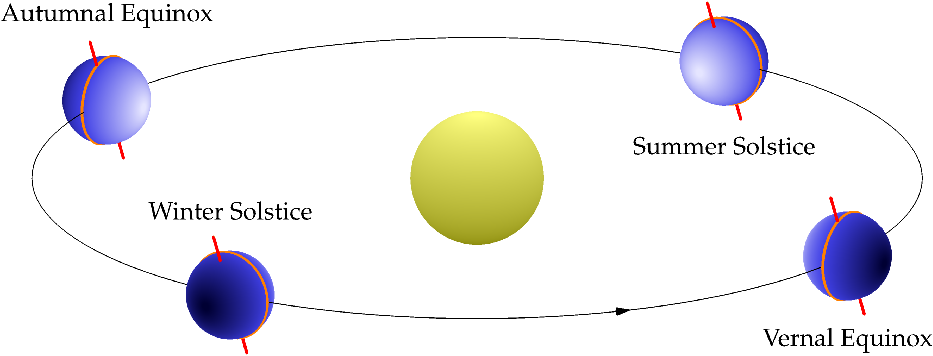
\includegraphics[scale=0.95]{ecliptic}}
\end{center}

Measurements can now be conducted relative to this set-up.

\begin{description}\itemsep0pt
  \item[\normalfont\emph{Fixed stars}] These form the background with respect to which everything else is measured. The \emph{ecliptic} is the sun's apparent path over the year set against the fixed stars. Planets (\emph{wandering stars}) are also seen to move relative to this background.
  \item[\normalfont\emph{Celestial longitude}] Measured from zero to \ang{360} around the ecliptic with \ang 0 at the vernal equinox. One degree corresponds approximately to the sun's apparent daily motion. The ecliptic is divided into twelve equal segments: Aries is 0--\ang{30} (March to April 21\st); Taurus is 30--\ang{60}, etc.
  \item[\normalfont\emph{Celestial latitude}] Measured in degrees north or south of the ecliptic; the sun has latitude zero.
\end{description}

This formulation was largely co-opted by the Greeks from Babylon. The Greeks kept the Babylonian base-60 degrees-minutes-seconds system, which, with minor modifications, persists to this day.\footnote{In modern times latitude and longitude (declination/right-ascension) are measured with respect to the earth's equatorial plane rather than the ecliptic. Such \emph{equatorial co-ordinates} are first known to have been introduced by Hipparchus of Nicaea (below). Right-ascension is measured in \emph{hours-minutes-seconds} rather than degrees, with 24 hours $=\ang{360}$, though modern scientific practice is to use decimals rather than the sexagesimal minutes and seconds.}

\goodbreak

\boldsubsubsection{The Circumference of the Earth}\phantomsection\label{pg:syene}

Eratosthenes of Cyrene (c.\,200\BC, pg.\,\pageref{pg:eratosthenes}) performed one of the earliest accurate estimations of the circumference of the earth. His idea was to measure the sun's rays at noon in two different places.\par
\begin{minipage}[t]{0.6\linewidth}\vspace{-5pt}
	\begin{itemize}\itemsep0pt
	  \item Syene (modern-day Aswan, Egypt) is approximately 5,000 \emph{stadia} south of Alexandria.
		\item When the sun is directly overhead at Syene, it is inclined $\ang 712'=\frac 1{50}\cdot \ang{360}$ at Alexandria.
		\item Earth's circumference is therefore approximately $50\cdot 5,000=250,000$ stadia.
	\end{itemize}
\end{minipage}
\hfill
\begin{minipage}[t]{0.39\linewidth}\vspace{-5pt}
	\flushright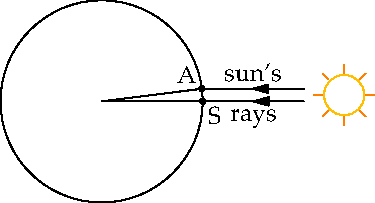
\includegraphics[scale=0.95]{geo-18-circearth}
\end{minipage}
\bigbreak

Eratosthenes' original calculation is lost, though it was a little more complicated than the above. From other (shorter) distances, historians have inferred that Eratosthenes' \emph{stadion} was $\approx 172$ yards, making his approximation for the circumference of the earth $\approx 24,500$ miles, astonishingly accurate in comparison to the modern value of $\approx 25,000$ miles. Later mathematicians provided other estimates based on other locations, but the basic method was the same.


\boldsubsubsection{Modelling the Heavens}

Early Greek analysis reflects several assumptions.
\begin{itemize}
  \item Spheres and circles are perfect, matching the `perfect design' of the universe. The earth is a sphere and the fixed stars (constellations) lie on a larger `celestial sphere.' Models relied on spheres and circles rotating at constant rates.
  \item The earth is stationary, so the celestial sphere rotates around it once per day.
  \item The planets lie on concentric spherical shells also centered on the earth.
\end{itemize}

When such assumptions are tested by observation, two major contradictions are immediate:
\begin{description}
  \item[\normalfont\emph{Variable brightness}] The apparent brightness of heavenly bodies, particularly planets, is not constant.
  \item[\normalfont\emph{Retrograde motion}] Planets mostly follow the east-west motion of the heavens, though are sometimes seen to slow down and \href{http://math.uci.edu/~ndonalds/math184/retrograde.html}{reverse course.}
\end{description}

If planets are moving at constant speed around circles centered on the earth, then how can these phenomena be explained? The attempt to produce accurate models while `saving the phenomena' of spherical/circular motion led to the development of new mathematics.\medbreak

One of the earliest known models is due to Eudoxus of Knidos (c.\,370\BC, pg.\,\pageref{pg:eudoxus}). Eudoxus developed a concentric-sphere model where planets and the sun are attached to separate spheres, each of which has its poles attached to the sphere outside it; the outermost sphere is that of the fixed stars. The motion generated by \href{http://web.calstatela.edu/faculty/hmendel/Ancient Mathematics/Eudoxus/Astronomy/EudoxusHomocentricSpheres.htm}{such a model}\footnote{The link is to a very nice flash animation of Eudoxus' model that would have been far beyond Eudoxus' ability to visualize and measure.} is highly complex. Eudoxus' approach is capable of producing retrograde motion, but not the variable brightness of stars and planets.
\goodbreak



\begin{minipage}[t]{0.74\linewidth}\vspace{0pt}
	\boldinline{Epicycles \& Eccentric Orbits} Apollonius of Perga (2\nd/3\rd{}\,C.\BC) is most famous for his study of conic sections, but is relevant in this section for developing two models for solar/planetary motion.\smallbreak
	
	In his \emph{eccenter} model, a planetary/solar orbit is a circle (the deferent) whose center is \emph{not} the earth. This straightforwardly addresses the problem of variable brightness since the planet is not a fixed distance from the earth.\smallbreak
	
	The obvious criticism is \emph{why?} What philosophical justification could there be for the eccenter? Eudoxus' model may have been complex and essentially impossible to compute with, but was more in line with the assumptions of spherical/circular motion.
\end{minipage}
\hfill
\begin{minipage}[t]{0.25\linewidth}\vspace{0pt}
  \flushright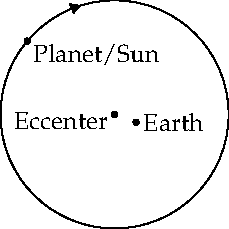
\includegraphics[scale=0.95]{trig-deferent}\phantom{b}
\end{minipage}
\medbreak
  

\begin{minipage}[t]{0.68\linewidth}\vspace{0pt}
	Apollonius' \href{http://brunelleschi.imss.fi.it/galileopalazzostrozzi/multimedia/ApolloniusEpicycles.html}{second approach} used \emph{epicycles}: small circles attached to a larger circle---you'll be familiar with epicycles if you've played with the toy \emph{Spirograph.} An observer at the center sees the apparent brightness change, and potentially observes retrograde motion. In modern language, the motion is parametrized by the vector-valued function
	\[
		\vx(t)=R\twovec{\cos \omega t}{\sin \omega t}+r\twovec{\cos \psi t}{\sin \psi t}
	\]
	where $R,r,\omega,\psi$ are the radii and frequencies (rad/s) of the circles.
\end{minipage}
\hfill
\begin{minipage}[t]{0.31\linewidth}\vspace{0pt}
  \flushright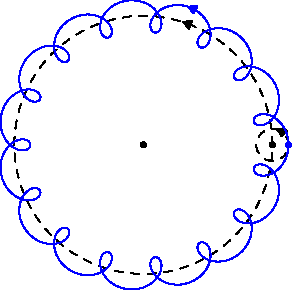
\includegraphics{trig-epicycle1}
\end{minipage}
\medbreak
  
Combining these models allowed Apollonius to describe very complex motion. Calculation was difficult however, requiring finding lengths of chords of various circles from a given angle, and vice versa. It is from this requirement that some of the earliest notions of trigonometry arise.\medbreak
 
One might ask why the Greeks didn't make the `obvious' fix and place the sun at the center of the cosmos. In fact Aristarchus of Samos (c.\,310--230\BC) did precisely this, suggesting that the fixed stars were really just other suns at exceptional distance! However, the great thinkers of the time (Plato, Aristotle, etc.) had a very strong objection to Aristarchus' approach: \emph{parallax.}
\begin{center}
	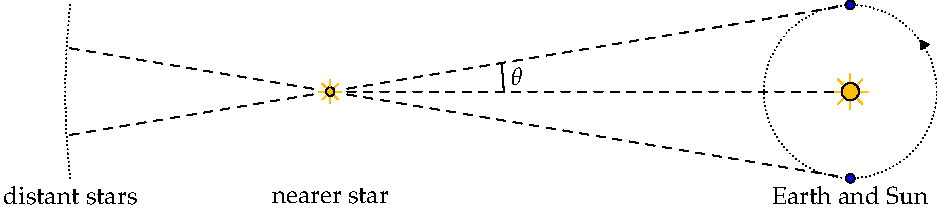
\includegraphics{trig-parallax}
\end{center}
If the earth moves around the sun and the fixed stars are really independent objects, then the position of a nearer star should appear to change throughout the year. The angle $\theta$ in the picture is the \emph{parallax} of the nearer star. Unfortunately for Aristarchus, the Greeks were incapable of observing any parallax.\footnote{The astronomical unit of one \emph{parsec} is the distance of a star exhibiting one arc-second ($\ang{\frac 1{3600}}$) of parallax, roughly 3.3 light-years or $3\times 10^{13}$\,km, an unimaginable distance to anyone before the scientific revolution. The nearest star to the sun is \emph{Proxima Centauri} at 4.2 light years $=0.77$ parsecs: is it any wonder the Greeks rejected the hypothesis?!}
It took 2000 years before the work of Copernicus and Kepler in the 15-1600s forced astronomers to take \emph{heliocentric} models seriously (\emph{Helios} is the Greek sun-god).
\goodbreak


\boldsubsubsection{Hipparchus of Nicaea/Rhodes (c.\,190--120\BC)}

Born in Nicaea (northern Turkey) but doing much of his work on the Mediterranean island of Rhodes, Hipparchus was one of the pre-eminent Greek astronomers. He made use of Babylonian eclipse data to fit Apollonius' eccenter and epicycle models to the observed motion of the moon. As part of this work, he needed to be able to accurately compute chords of circles; his resulting \emph{chord tables} are acknowledged as the earliest tables of trigonometric values.\par

\begin{minipage}[t]{0.63\linewidth}\vspace{0pt}
	In an imitation of Hipparchus' approach, we define a function crd which returns the length of the chord in a given circle subtended by a given angle. Translated to modern language,
	\[
		\crd\alpha=2r\sin\frac\alpha 2
	\]
\end{minipage}
\hfill
\begin{minipage}[t]{0.36\linewidth}\vspace{-10pt}
	\flushright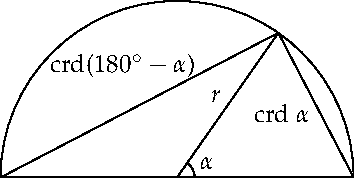
\includegraphics[scale=0.95]{trig-chord}
\end{minipage}\medbreak
Hipparchus chose a circle with circumference \ang{360} (in fact he used $60\cdot 360=21600$ arc-minutes), the result being that $r=\frac{21600}{2\pi}\approx 57,18$ (written base 60!). Note that this is sixty times the number of \emph{degrees per radian.}\footnote{One radian is the angle subtended by an arc equal in length to the radius of a circle. Hipparchus essentially does this in reverse; the circumference is fixed so that \emph{degree} now measures both subtended angle \emph{and} circumferential distance.} His chord table was constructed starting with two obvious values:
\[
	\crd \ang{60}=r=57,18\qquad \crd \ang{90}=\sqrt 2r=81,2
\]
Since (Thales) the large triangle is right-angled, the Pythagorean theorem was used to obtain chords for angles $\ang{180}-\alpha$. In modern language
\[
	\crd(\ang{180}-\alpha) =\sqrt{(2r)^2-(\crd\alpha)^2} =2r\sqrt{1-\sin^2(\alpha/2)} =2r\cos\frac\alpha 2
	\]
Pythagoras was again used to halve and double angles in an approach analogous to Archimedes' quadrature of the circle (pg.\,\pageref{pg:archquadcircle}). We rewrite the argument in this language.\par
\begin{minipage}[t]{0.6\linewidth}\vspace{0pt}
	In the picture, we double the angle $\alpha$; plainly $M$ is the midpoint of $\cl{AD}$ and $\nm{DB}=\crd(\ang{180}-2\alpha)$. Since $\angle BDA=\ang{90}$, it follows that $\cl{BD}$ is parallel to $\cl{OM}$ and so
	\[
		\nm{OM}=\frac 12\nm{BD}=\frac 12\crd(\ang{180}-2\alpha)
	\]
	Now apply Pythagoras to $\triangle CMD$:
\end{minipage}
\hfill
\begin{minipage}[t]{0.39\linewidth}\vspace{0pt}
	\flushright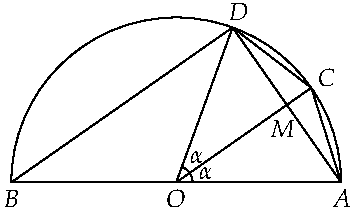
\includegraphics[scale=0.95]{trig-double}
\end{minipage}
\begin{align*}
	\left(\crd\alpha\right)^2&=\left(\frac 12\crd 2\alpha\right)^2+\left(r-\frac 12\crd(\ang{180}-2\alpha)\right)^2 \tag{$\nm{CD}^2=\nm{DM}^2+\nm{CM}^2$}\\
	&=\frac 14(\crd 2\alpha)^2+r^2-r\crd(\ang{180}-2\alpha)+\frac 14\crd(\ang{180}-2\alpha)^2\\
	&=\frac 14(\crd 2\alpha)^2+r^2-r\crd(\ang{180}-2\alpha)+\frac 14(4r^2-(\crd 2\alpha)^2)\\
	&=2r^2-r\crd(\ang{180}-2\alpha)
\end{align*}
In modern notation this is one of the double-angle trigonometric identities!
\[
	4r^2\sin^2\frac\alpha 2 =2r^2-2r^2\cos\alpha\iff \cos\alpha=1-2\sin^2\frac\alpha 2
\]
\goodbreak


\boldinline{Example} To calculate $\crd \ang{30}$, we start with $\crd\ang{60}=r$. Then
\begin{align*}
	&\crd\ang{120}=\sqrt{4r^2-r^2}=\sqrt 3\,r\\
	\implies &\crd\ang{30}=\sqrt{2r^2-r\crd(\ang{180}-\ang{60})}=\sqrt{2r^2-\sqrt 3r^2}=\sqrt{2-\sqrt 3}\,r
\end{align*}
In modern language this yields an exact value for $\sin\ang{15}$:
\[
	\crd\ang{30}=2r\sin\ang{15}\implies\sin\ang{15} =\frac 12\sqrt{2-\sqrt 3}
\]
Continuing this process, we obtain $\crd \ang{150}=\sqrt{2+\sqrt 3}\,r$, whence
\[
	\crd\ang{15})^2=2r^2-r\crd\ang{150}=(2-\sqrt{2+\sqrt 3})\,r\implies \crd\ang{15}=\sqrt{2-\sqrt{2+\sqrt 3}}\,r
\]
Again translating: $\sin\ang{7.5}=\frac 12\sqrt{2-\sqrt{2+\sqrt 3}}$.\smallbreak

By applying this approach, Hipparchus computed the chord of each of the angles $\ang{7.5}$, $\ang{15},\ldots,\ang{172.5}$, in steps of $\ang{7.5}$. Of course everything was an estimate since he had to rely on approximations for square-roots. All Hipparchus' original work is now lost. We primarily know of his work by reference. In particular, the above method of chords is probably due to Hipparchus, although we see it first in the work of Ptolemy, as we'll consider next.



\begin{exercises}{}{}
	\exstart %[5-2]
	Calculate $\crd\ang{150}$, $\crd\ang{165}$, and $\crd\ang{172\tfrac 12}$ using the method of Hipparchus.\vspace{-5pt}
	\begin{enumerate}\setcounter{enumi}{1}
	  \item[](\emph{Leave your answers as a multiple of $r=\crd\ang{60}$})
	  
	  \item \emph{Sirius,} the brightest star in the sky, is 2.64 parsecs (8.6 light-years) from the sun. Use modern trigonometry to find its parallax.
	
		\item\label{exs:tropicstick1} The tropic of cancer is the line of latitude (approximately) \ang{23.5} north of the equator marking the locations where the sun is directly overhead at noon on the summer solstice.\footnotemark{} At the arctic circle on the \emph{winter} solstice, the sun is precisely on the horizon.
		\begin{enumerate}
		  \item Explain why the latitude of the arctic circle is \ang{66.5} north.
		  \item Find the angle the sun makes \emph{above} the horizon at the arctic circle at noon on the summer solstice.
		\end{enumerate}
	  
	  \item Consider the epicycle model where the position vector of a planet is given by
	  \[
	  	\vx(t)=R\twovec{\cos \omega t}{\sin \omega t}+r\twovec{\cos \psi t}{\sin \psi t}
	  \]
	  \begin{enumerate}
	    \item Suppose $R=4$ and $r=1$, $\omega=1$ and $\psi=2$, so that the epicycle rotates twice every orbit. Sketch a picture of the full orbit.
	    \item Suppose that $\omega,\psi$ are positive constants. Prove that an observer will see retrograde motion if and only if $r\psi>R\omega$.\par
	  	(\emph{Hint: differentiate $\vx'(t)$ and think about its direction})
	  \end{enumerate}
	\end{enumerate}
\end{exercises}

\footnotetext{Syene (pg.\,\pageref{pg:syene}) is almost exactly on the Tropic of Cancer.}

\clearpage


\subsection{Ptolemy's \emph{Almagest}}

Born in Egypt and living much of his life in Alexandria, Claudius Ptolemy (c.\,\AD 100--170) was a Greek/Egyptian/Roman\footnote{Ptolemy (Ptolemaeus) is a Greek name, while Claudius is Roman, reflecting the changing cultural situation in Egypt.} astronomer and mathematician. Around \AD 150, he produced the \emph{Mathematica Syntaxis,} better known as the \emph{Almagest}; the latter term is derived from the Arabic \emph{al-mageisti} (great work), reflecting its importance to later Islamic learning.\par
 
The \emph{Almagest} is essentially a textbook on geocentric cosmology. It shows how to compute the motions of the moon, sun and planets, describing lunar parallax, eclipses, the constellations, and elementary spherical trigonometry, probably courtesy of Menelaus (c.\,\AD 100). It contains our best evidence as to the accomplishments of Hipparchus and describes his calculations. The text formed the basis of Western/Islamic astronomical theory through the 1600s.


\boldinline{Ptolemy's Calculations}

Ptolemy used several innovations to compute more chords and at a far greater accuracy than Hipparchus.

\begin{description}
	\item[\normalfont\emph{Initial Data}] Ptolemy took $r=60$ so that $\crd\ang{60}=60$. He also had more initial data: 
	\[
		\crd\ang{90}=60\sqrt 2,
		\quad
		\crd\ang{36}=30(\sqrt 5-1),
		\quad
		\crd\ang{72}=30\sqrt{10-2\sqrt 5}
	\]
	\item[\normalfont\emph{Halving/Doubling Angles}] Ptolemy used what was probably Hipparchus' method:
	\begin{gather*}
	  \crd^2\alpha=2r^2-r\crd(\ang{180}-2\alpha)=60\big(120-\crd(\ang{180}-2\alpha)\big)\\
	  \crd(\ang{180}-\alpha)=\sqrt{(2r)^2-\crd^2\alpha}=\sqrt{120^2-\crd^2\alpha}
	\end{gather*}
	with square-roots approximated to the desired accuracy. For example,
	\[
	  \crd\ang{30}=\sqrt{60(120-\crd \ang{120})}=\sqrt{60\left(120-60\sqrt 3\right)}=60\sqrt{2-\sqrt 3}\approx 31;3,30
	\]
	\item[\normalfont\emph{Multiple-Angle Formula}] Ptolemy computed $\crd\ang{12}=\crd(\ang{72}-\ang{60})$, then halved this for angles of \ang 6, \ang 3, \ang{1.5}, and \ang{0.75}. Chords for all integer multiples of \ang{1.5} were computed using addition formula.
	\item[\normalfont\emph{Interpolation}] The observation %\footnote{In modern language $x<y\implies\frac{\sin y}y<\frac{\sin x}x$ so that $\frac{\sin x}x$ increases to 1 as $x\to 0^+$.}
	$\alpha<\beta\Longrightarrow \frac{\crd\beta}{\crd\alpha}<\frac\beta\alpha$ allowed Ptolemy to compute chords for every half-degree to the incredible accuracy of two sexagesimal places. For approximating between half-degrees, his table indicated how much should be added for each arc-minute ($\ang{\frac 1{60}}$). For example, the second line of Ptolemy's table reads
	\[
		\ang 1\qquad 1;2,50\qquad ;1,2,50
	\]
	The first two columns state that $\crd\ang 1= 1;2,50$ to two sexagesimal places.\footnote{This is $1+\frac 2{60}+\frac{50}{60^2}=1.0472222\ldots=120\sin\ang{\frac{1.00003625\ldots}2}$, an already phenomenal level of accuracy.} The third entry says, for example, that
	\[
		\crd \ang{1}5'\approx 1;2,50+5(;1,2,50)=1;8,4,10\approx 1;8;4
	\]
	To obtain these arc-minute approximations, it is believed Ptolemy computed half-angle chords to an accuracy of \emph{five sexagesimal places} (1 part in over 750 million!).
\end{description} 

\goodbreak



\boldinline{How did Ptolemy know the values of $\crd \ang{36}$ and $\crd \ang{72}$?}

Everything necessary is in the \emph{Elements.}

\begin{thm*}{}{}
	\exstart (Thm XIII.\,9)\lstsp In a circle, the sides of a regular inscribed hexagon and decagon are in the golden ratio (this ratio is\ $60:\crd \ang{36}$ in Ptolemy).
	\begin{enumerate}\setcounter{enumi}{1}
	  \item (Thm XIII.\,10)\lstsp In a circle, the square on an inscribed pentagon equals the sum of the squares on an inscribed hexagon and decagon.
	\end{enumerate}
\end{thm*}

Purely Euclidean proofs are too difficult for us, so here is a way to see things in modern notation.

\begin{minipage}[t]{0.55\linewidth}\vspace{0pt}
	\begin{enumerate}
	  \item Let $\textcolor{blue}{\cl{AB}}=\textcolor{blue}{x}$ be the side of a regular decagon inscribed in a unit circle with center $O$.\par
	  $\triangle OAB$ is isosceles with angles $\ang{36}$, $\ang{72}$, $\ang{72}$.\par
		Let $C$ lie on $\cl{OB}$ such that $\cl{AC}=x$.\par
		Count angles to see that $\triangle OAB$ and $\triangle ABC$ are similar, that $\angle OAC=\ang{36}$ and so $\cl{OC}=x$.\par
		Similarity now tells us that
		\[
			x=\frac{1-x}x\implies x=\dfrac{\sqrt 5-1}2
		\]
		In a circle of radius 60, this gives the exact value
	  \[
	  	\crd \ang{36}=60x=30(\sqrt 5-1)
	  \]
	  \end{enumerate}
\end{minipage}
\hfill
\begin{minipage}[t]{0.44\linewidth}\vspace{0pt}
	\flushright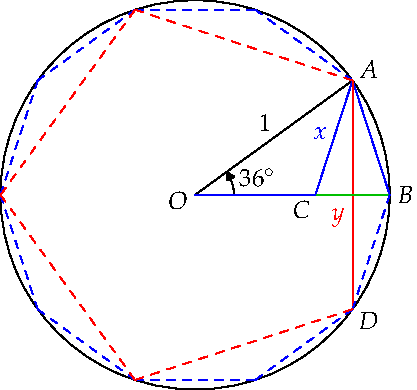
\includegraphics[scale=0.95]{pentagon}
\end{minipage}

\begin{enumerate}\setcounter{enumi}{1}
  \item Now let $\textcolor{red}{\cl{AD}}=\textcolor{red}{y}$ be the side of a regular pentagon inscribed in the same circle. Applying Pythagoras, we see that
  \[
  	\left(\textcolor{red}{\frac y2}\right)^2+\left(\textcolor{Green}{\frac{1-x}2}\right)^2=\textcolor{blue}{x}^2
  \]
  Since $x^2=1-x$, this multiplies out to give Euclid's result
  \[
  	y^2=1^2+x^2
  \]
  from which we obtain the exact value
  \[
  	\crd\ang{72}=60y=30\sqrt{10-2\sqrt 5}
  \]
\end{enumerate}
  
While these values were geometrically precise, Ptolemy used sexagesimal approximations to square-roots to obtain
\[
	\crd\ang{36} =37;4,55\qquad \crd\ang{72}=70;32,3
\]
While these are the values stated in his tables, he must have used a far higher degree of accuracy in order to obtain similarly accurate values for other chords.
\goodbreak


\boldinline{Angle-addition}

Computation of $\crd(\alpha\pm\beta)$ was facilitated by versions of the multiple-angle formulæ of modern trigonometry.

\begin{thm*}{Ptolemy's Theorem}{}
	Suppose a quadrilateral is inscribed in a circle. Then the product of the diagonals equals the sum of the products of the opposite sides.\footnotemark
\end{thm*}\phantomsection\label{pg:ptolemythm}

\footnotetext{It is generally considered that this result predates Ptolemy, though there is some debate as to whether it belongs in the \emph{Elements.} Book VI traditionally contains 33 propositions, however some editions append four corollaries, of which Ptolemy's Theorem is the last (Thm VI.\,D).}

\begin{proof}
	Choose $E$ on $\cl{AC}$ such that $\angle ABE\cong\angle DBC$. Then $\angle ABD\cong\angle EBC$. Since $\angle BAE\cong\angle BDC$ are inscribed angles of the same arc $\cl{BC}$, we obtain two pairs of similar triangles:
	\begin{center}
		\begin{tabular}{c@{\qquad\qquad}c}
			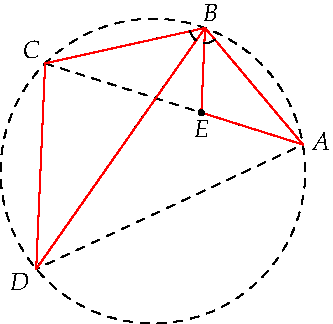
\includegraphics[scale=1]{ptolemy1}
			&
			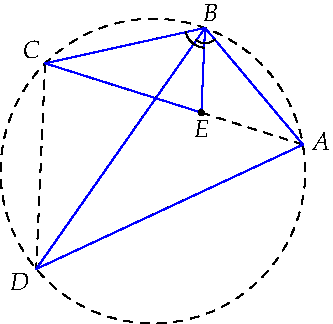
\includegraphics[scale=1]{ptolemy2}
			\\
			$\triangle ABE\sim\triangle DBC$
			&
			$\triangle ABD\sim\triangle EBC$
		\end{tabular}
	\end{center}
	The proof follows immediately: since $\frac{\nm{AE}}{\nm{CD}}=\frac{\nm{AB}}{\nm{BD}}$ and $\frac{\nm{CE}}{\nm{AD}}=\frac{\nm{BC}}{\nm{BD}}$, we have
	\[
		\nm{AC}\nm{BD}=(\nm{AE}+\nm{CE})\nm{BD}=\nm{AB}\nm{CD}+\nm{AD}\nm{BC} \tag*{\qedhere}
	\]
\end{proof}


\begin{cor*}[lower separated=false, sidebyside, sidebyside align=top seam, sidebyside gap=0pt, righthand width=0.34\linewidth]{}{}
	If $\alpha>\beta$, then
	\[
		120\crd(\alpha-\beta)=\crd\alpha\crd(\ang{180}-\beta)-\crd\beta\crd(\ang{180}-\alpha)
	\]
	In modern language, divide out by $120^2$ to obtain
	\[
		\sin\frac{\alpha-\beta}2=\sin\frac\alpha 2\cos\frac\beta 2-\sin\frac\beta 2\cos\frac\alpha 2
	\]
	\tcblower
	\flushright
	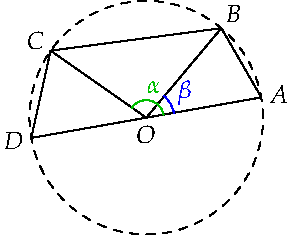
\includegraphics[scale=0.9]{trig-multiple}
\end{cor*}


\begin{proof}
	If $\nm{AD}=120$ is a diameter of the pictured circle, then Ptolemy's Theorem says
	\[
		\crd\alpha\crd(\ang{180}-\beta)=\crd\beta\crd(\ang{180}-\alpha)+120\crd(\alpha-\beta) \tag*{\qedhere}
	\]
\end{proof}

Similar expressions for $\crd(\alpha+\beta)$ and $\crd(\ang{180}-(\alpha\pm\beta))$ were also obtained, essentially recovering all versions of the multiple-angle formulæ for $\sin(\alpha\pm\beta)$ and $\cos(\alpha\pm\beta)$.
\goodbreak


\boldinline{Examples}
	\exstart Here is how Ptolemy might have calculated $\crd \ang{42}$. Let $\alpha=\ang{72}$ and $\beta=\ang{30}$, then
	\[
		120\crd \ang{42}=\crd\ang{72}\crd\ang{150}-\crd\ang{30}\crd \ang{108}
	\]
	Since $\crd \ang{72}=30\sqrt{10-2\sqrt 5}$ is known, and
	\[
		\crd \ang{108}=\crd(\ang{180}-\ang{72})=\sqrt{120^2-\crd^2\ang{72}}=30\sqrt{6+2\sqrt 5}
	\]
	we see that
	\begin{align*}
		\crd \ang{42}&=\frac 1{120}\left(30\sqrt{10-2\sqrt 5}\cdot 60\sqrt{2+\sqrt 3} -60\sqrt{2-\sqrt 3} \cdot 30\sqrt{6+2\sqrt 5}\right)\\
		&=15\left(\sqrt{10-2\sqrt 5}\cdot \sqrt{2+\sqrt 3} -\sqrt{2-\sqrt 3} \cdot \sqrt{6+2\sqrt 5}\right) \approx 43;0,15\approx 43.0042
	\end{align*}
	Note all the square-roots which had to be approximated. The construction of the chord-table was truly a gargantuan task, one for which Ptolemy almost certainly had assistance.
	
	\begin{enumerate}\setcounter{enumi}{1}
	  \item The \emph{Almagest} also contained many practical examples. Here is one such.\par
		\begin{minipage}[t]{0.65\linewidth}\vspace{-10pt}
			A stick of length 1 is placed in the ground. The angle of elevation of the sun is \ang{72}. What is the length of its shadow?\smallbreak
		
			Ptolemy instructs the reader to draw a picture. The lower isosceles triangle has \textcolor{blue}{base angles} \ang{72}, and the length of the shadow $\ell$ is marked. Even though the circle does not have radius 60, the ratio of the chords may be computed:
			\begin{align*}
				&1:\ell=\crd \textcolor{orange}{\ang{144}}:\crd \textcolor{Green}{\ang{36}}\\
				\implies &\ell=\frac{\crd \ang{36}}{\crd \ang{144}}=\frac{30(\sqrt 5-1)}{30\sqrt{10+2\sqrt 5}}\approx 0.32491
			\end{align*}
			This is precisely $\cot \ang{72}$, though Ptolemy had no such notion.
		\end{minipage}
		\hfill
		\begin{minipage}[t]{0.34\linewidth}\vspace{-5pt}
			\flushright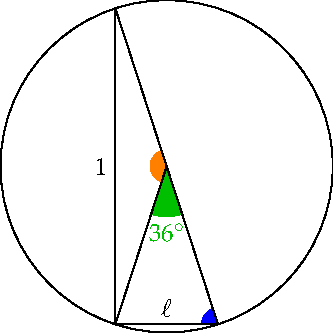
\includegraphics[scale=0.9]{trig-anglesun}
		\end{minipage}
	\end{enumerate}



%Further calculations and examples were far more complex!\smallbreak

% It is worth noting that Ptolemy's system was resolutely \emph{geocentric.} Similarly to how the fame of Euclid's \emph{Elements} shaped 2000 years of mathematical principle, the massive impact of Ptolemy's \emph{Almagest} and the reverence felt for ancient knowledge meant that it became increasingly difficult in medieval Europe to challenge geocentrism.



\begin{exercises}{}{}
	\exstart What are the exact values of $\sin\ang{36}$ and $\sin\ang{18}$?
	
	\begin{enumerate}\setcounter{enumi}{1}
	  \item\begin{enumerate}
	    \item Rewrite Ptolemy's interpolation formula $\alpha<\beta\Longrightarrow \frac{\crd\beta}{\crd\alpha}<\frac\beta\alpha$ in terms of the sine function. What facts about $\frac{\sin x}x$ does this reflect?
	    \item Find $\crd 57'$ (arc-minutes!) to two sexagesimal places.
	  \end{enumerate} 
	  
	  \item Find the exact value of $\crd \ang{54}$
	  
	  \item%[5-4]
	  Prove the following using Ptolemy's Theorem. What is this in modern language?
	  \[
	  	120\crd\bigl(\ang{180}-(\alpha+\beta)\bigr) =\crd(\ang{180}-\alpha)\crd(\ang{180}-\beta)-\crd\alpha\crd\beta
	  \]
	  
	  
	  \item%[5-8]
	  Calculate the length of a noon shadow of a pole of length 60 using Ptolemy's methods:
	  \begin{enumerate}
	    \item On the vernal equinox at latitude $\ang{40}$.
	  	\item%[5-10](Hard!)\lstsp
	  	At latitude \ang{36} north on both the summer and winter solstices.\par
	  (\emph{Hint: recall Exercise \ref*{ssec:astro1}.\ref{exs:tropicstick1}})
	  \end{enumerate}
	\end{enumerate}
\end{exercises}